\documentclass[a4paper,10pt]{article}
\usepackage{multirow}
\usepackage{graphicx}
\usepackage{fancyhdr}
\usepackage{lastpage}
\usepackage{amssymb}
\usepackage{epsfig}
\usepackage{latexsym}
\usepackage{amstext}
\usepackage{amsmath}
\usepackage{amsfonts}
\usepackage{amsthm}
\usepackage{array}
\usepackage{tikz}
\usepackage{fancyvrb}
\usepackage[a4paper, total={6.5in, 10in}]{geometry}
\usepackage{indentfirst}
\usepackage[T1]{fontenc}
\usepackage[sc]{mathpazo}

\newcommand{\BigO}[1]{\ensuremath{\textrm{O}\left(#1\right)}}
\newcommand{\Nat}{\ensuremath{\mathbb{N}}}
\newcommand{\Real}{\ensuremath{\mathbb{R}}}
\newcommand{\SSort}{\textsc{Slowsort }}
\newcommand{\Arrow}[1]{\ensuremath{\xrightarrow{\hspace*{#1 cm}}}}
\newcommand{\floor}[1]{\ensuremath{\left\lfloor #1 \right\rfloor}}

\title{Runtime analysis of the \SSort algorithm}
\author{Lucio Santi\\
\small{lsanti at dc.uba.ar}}
\date{}

\begin{document}
\pagestyle{fancyplain}
\cfoot{- \thepage/\pageref{LastPage} -}
\lhead{}
\chead{}
\rhead{}
\renewcommand{\headrulewidth}{0pt}

\maketitle

\section{Introduction}

\indent This document provides a runtime analysis of the \SSort algorithm\cite{SS}. Despite being presented in a satirical article, its recursion pattern turns out to be rather complex, which in turn makes it harder to analyze. On the other hand, the authors do not provide a thorough derivation of the claimed running time in the aforementioned article. The asymptotic bounds explored here do not match tightly with those, as they differ roughly by a linear factor.

\section{\SSort algorithm}

\indent The following figure shows the pseudocode of \SSort:

    \begin{center}
    \framebox[7.5cm]{
    \begin{minipage}{7.5cm}
        \setlength{\parindent}{15pt}
        \vspace{0.2cm}
        \SSort($A[1 \dots n]$):\\
        \hspace*{1cm} If $n = 1$: return.\\
        \hspace*{1cm} Let $m := \frac{n+1}{2}$.\\
        \hspace*{1cm} \SSort($A[1 \dots m]$).\\
        \hspace*{1cm} \SSort($A[m+1 \dots n]$).\\   
        \hspace*{1cm} If $A[n] < A[m]$: swap $A[n]$ and $A[m]$.\\
        \hspace*{1cm} \SSort($A[1 \dots n-1]$).             
        \vspace{0.2cm}
    \end{minipage}}
    \end{center}


\section{Runtime analysis}

\subsection{Recurrence relation}

Let $T(n)$ be the function that characterizes the worst-case running time of \SSort when given an input array of size $n$. Being a recursive algorithm, we can define $T$ recurrently like so:

$$T(n) = 2T(n/2) + T(n-1) + \Theta(1)$$

\vspace{0.1cm}
Note that we intentionally leave out base cases as we aim at finding asymptotic bounds for $T$. From this, we can see that $T(i) - T(i-1) = 2T(i/2) + \Theta(1)$ for a given $i$. Thus,

\begin{alignat*}{2}
    &\quad \displaystyle \sum_{i = 1}^{n}{T(i) - T(i-1)} \, &= & \,\, \displaystyle \sum_{i = 1}^{n}{2T(i/2) + \Theta(1)} \\
    &\Rightarrow \quad T(n) - T(0) &=& \,\, \displaystyle \sum_{i = 1}^{n}{2T(i/2)} + \displaystyle \sum_{i = 1}^{n}{\Theta(1)} \\
    &\Rightarrow \quad T(n) - T(0) &=& \,\, \displaystyle \sum_{i = 1}^{n}{2T(i/2)} + \Theta(n) \\
    &\Rightarrow \quad\quad\quad T(n) &=& \,\, \displaystyle \sum_{i = 1}^{n}{2T(i/2)} + \Theta(n) \\
\end{alignat*}

\subsection{Asymptotic bounds}

We shall look now for asymptotic bounds for $T$. Let us consider first the following recurrence $U$:

\begin{eqnarray*}
    U(n) &=& \displaystyle \sum_{i = 1}^{n}{2U(n/2)} + \Theta(n) \\
         &=& 2n \, U(n/2) + \Theta(n)
\end{eqnarray*}

Clearly, we have that $T(n) \leq U(n)$ for all $n$. In order to find an asymptotic solution for $U$, let's have a look at its recursion tree:\\

\hspace{-0.5cm}
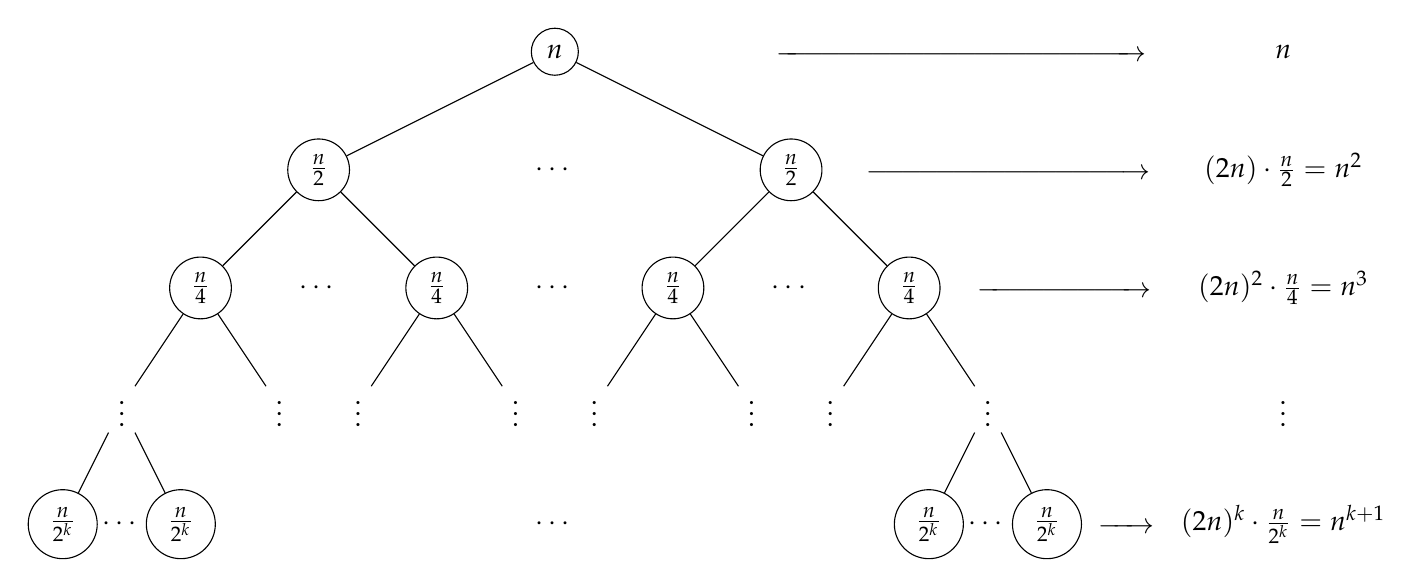
\begin{tikzpicture}[level/.style={sibling distance=60mm/#1}]
\node [circle,draw] (z){$n$}
  child {node [circle,draw] (a) {$\frac{n}{2}$}
    child {node [circle,draw] (b) {$\frac{n}{4}$}
      child {node {$\vdots$}
        child {node [circle,draw] (d) {$\frac{n}{2^k}$}}
        child {node [circle,draw] (e) {$\frac{n}{2^k}$}}
      } 
      child {node {$\vdots$}}
    }
    child {node [circle,draw] (g) {$\frac{n}{4}$}
      child {node {$\vdots$}}
      child {node {$\vdots$}}
    }
  }
  child {node [circle,draw] (j) {$\frac{n}{2}$}
    child {node [circle,draw] (k) {$\frac{n}{4}$}
      child {node {$\vdots$}}
      child {node {$\vdots$}}
    }
  child {node [circle,draw] (l) {$\frac{n}{4}$}
    child {node {$\vdots$}}
    child {node (c){$\vdots$}
      child {node [circle,draw] (o) {$\frac{n}{2^k}$}}
      child {node [circle,draw] (p) {$\frac{n}{2^k}$}
        child [grow=right] {node (q3) {} edge from parent[draw=none]
          child [grow=right] {node (q) {$(2n)^k \cdot \frac{n}{2^k} = n^{k+1}$} edge from parent[draw=none]
            child [grow=up] {node (r) {$\vdots$} edge from parent[draw=none]
              child [grow=up] {node (s) {$(2n)^2 \cdot \frac{n}{4} = n^3$} edge from parent[draw=none]
                child [grow=up] {node (t) {$(2n) \cdot \frac{n}{2} = n^2$} edge from parent[draw=none]
                  child [grow=up] {node (u) {$n$} edge from parent[draw=none]}
                }
              }
            }
          }
        }
      }
    }
  }
};

\path (a) -- (j) node [midway] {$\cdots$};

\path (b) -- (g) node [midway] {$\cdots$};
\path (g) -- (k) node [midway] {$\cdots$};
\path (k) -- (l) node [midway] {$\cdots$};

\path (d) -- (e) node [midway] {$\cdots$};
\path (o) -- (p) node [midway] {$\cdots$};

\path (o) -- (e) node (x) [midway] {$\cdots$};

\path (z) -- (u) node [midway] {$\hspace{1cm} \Arrow{4.5}$};
\path (s) -- (l) node [midway] {$\Arrow{2}$};
\path (j) -- (t) node [midway] {$\Arrow{3.4}$};
\path (p) -- (q) node [midway] {$\Arrow{0.5}$};
\end{tikzpicture}

\vspace{1cm}

From this, it follows that

\begin{eqnarray*}
    U(n) &=& \displaystyle \sum_{k = 0}^{\floor{\log_2(n)}}{n^{k+1}} \\
         &=& n \, \displaystyle \sum_{k = 0}^{\floor{\log_2(n)}}{n^k} \\
         &=& \frac{n}{n-1} \, \left(n^{\floor{\log_2(n)} + 1} - 1 \right) \\
         &\in& \Theta \left(n^{\log_2(n) + 1} \right)
\end{eqnarray*}

This yields an asymptotic upper bound for $T$:

\begin{equation}
\label{eq:bigO}
    T(n) \in \BigO{n^{\log_2(n) + 1}}
\end{equation}

In order to find an asymptotic lower bound, let's first rewrite $T$ in the following convenient way:

\begin{equation*}
    T(n) = \displaystyle \sum_{i = 0}^{n-1}{2T(n/2 - i/2)} + \Theta(n)
\end{equation*} 

Now, let us choose an arbitrary $\alpha \in \Real$ such that $0 < \alpha < 1$ and define the recurrence $L_{\alpha}(n)$ as follows:

\begin{equation*}
    L_{\alpha}(n) = \displaystyle \sum_{i = 0}^{\floor{n^{\alpha}} - 1}{2L_{\alpha}(n/2 - i/2)} + \Theta(n)
\end{equation*}

Such an $L_{\alpha}$ nearly satisfies every hypotheses required by the Akra-Bazzi theorem\cite{AB}. The only apparent exception is that the summation in the right-hand side goes up to a function of $n$, and the theorem states that this value should be a constant $k \in \Nat$. However, the proof outlined in \cite{AB} does not seem to rely strongly on this fact\footnote{If someone sufficiently qualified to confirm or disprove this assertion ever reads this, please let me know. Thanks in advance!}. In what follows, then, we will use the Akra-Bazzi theorem to obtain an asymptotic solution for $L$.\\

Before proceeding, we observe that the index perturbation functions $h_i(n)$ are properly bounded:

\begin{eqnarray}
\label{eq:h}
    |h_i(n)| &=& |-\frac{i}{2}| \nonumber \\
             &=& \frac{i}{2} \nonumber \\
             &\leq& \frac{n^{\alpha} - 1}{2} \nonumber \\
             &\leq& n^{\alpha} \nonumber \\
             &\in& \BigO{\frac{n}{\log^2{n}}}
\end{eqnarray}

(\ref{eq:h}) holds since $\frac{n^{\alpha}}{n / \log^2{n}}$ goes to $0$ as $n \rightarrow  \infty$.\\

Now, we need to find the value of $p$ to plug into the theorem and find a tight asymptotic bound for $L_{\alpha}$:

\begin{alignat*}{2}
    &\quad \,\, \displaystyle \sum_{i = 0}^{\floor{n^{\alpha}} - 1}{a_i b_i^p} \quad &= & \quad 1 \\ 
    &\Leftrightarrow \displaystyle \sum_{i = 0}^{\floor{n^{\alpha}} - 1}{2 \, \frac{1}{2^p}} \quad &=& \quad 1 \\
    &\Leftrightarrow  \quad\quad\quad \frac{\floor{n^{\alpha}}}{2^{p-1}}\quad &=& \quad 1 \\
    &\Leftrightarrow  \quad\quad \log_2\left(\floor{n^{\alpha}}\right) \quad &=& \quad p - 1 \\
    &\Leftrightarrow  \quad\quad\quad\quad p \quad &=& \quad \log_2\left(\floor{n^{\alpha}}\right) + 1 \\
\end{alignat*}

With this in hand, we can calculate the following integral:

\begin{eqnarray*}
    \int_{1}^{n}{\frac{g(x)}{x^{p+1}} \, dx} &=& \int_{1}^{n}{\frac{x}{x^{\log_2\left(\floor{n^{\alpha}}\right) + 2}} \, dx} \\
    &=& \int_{1}^{n}{\frac{dx}{x^{\log_2\left(\floor{n^{\alpha}}\right) + 1}}} \\
    &=& \frac{-1}{\log_2\left(\floor{n^{\alpha}}\right) \, x^{\log_2\left(\floor{n^{\alpha}}\right)}} \bigg\rvert_{1}^{n} \\
    &=& \frac{1}{\log_2\left(\floor{n^{\alpha}}\right)} - \frac{1}{\log_2\left(\floor{n^{\alpha}}\right) \, n^{\log_2\left(\floor{n^{\alpha}}\right)}}
\end{eqnarray*}

Finally,

\begin{eqnarray*}
    n^p \, \left(1 + \int_{1}^{n}{\frac{g(x)}{x^{p+1}} \, dx}\right) &=& n^{\log_2\left(\floor{n^{\alpha}}\right) + 1} \,
                                                                         \left(1 + \frac{1}{\log_2\left(\floor{n^{\alpha}}\right)}
                                                                         - \frac{1}{\log_2\left(\floor{n^{\alpha}}\right) \, n^{\log_2\left(\floor{n^{\alpha}}\right)}}
                                                                         \right) \\
    &\in& \Theta \left(n^{\log_2\left(\floor{n^{\alpha}}\right) + 1}\right) \\
    &=& \Theta \left(n^{\alpha \log_2(n) + 1} \right)
\end{eqnarray*}

Therefore,

$$L_{\alpha}(n) \in \Theta \left(n^{\alpha \log_2(n) + 1}\right)$$

which, since $L_{\alpha}(n) \leq T(n)$ for all $n$, implies that

\begin{equation}
\label{eq:omega}
    T(n) \in \Omega \left(n^{\alpha \log_2(n) + 1}\right)
\end{equation}

\vspace{1cm}

Putting everything together, it follows from (\ref{eq:bigO}) and (\ref{eq:omega}) that, for sufficiently large $n$, there exist some constants $c_1, c_2 > 0$ such that

$$c_1 \, n^{\alpha \log_2(n) + 1} \leq T(n) \leq c_2 \, n^{{\log_2(n) + 1}}$$

for any $\alpha \in (0, 1)$.

\subsection{Remarks about $\alpha$}

The lower bound we explored above is only valid when $0 < \alpha < 1$. We might be tempted to choose $\alpha = 1$ in order to obtain a tight asymptotic bound for $T$, but unfortunately doing so would violate the index perturbation hypothesis of the Akra-Bazzi theorem. Indeed, in such cases, $h_i(n) \leq \frac{n-1}{2}$, and thus some of these functions will not be bounded the way the theorem expects.

\bibliography{slowsort} 
\bibliographystyle{ieeetr}

\end{document}
